\chapter{Estado del arte}\label{EdA}
%Función que crea el título de capítulo y al cual se le da el nombre deseado a través de su parámetro obligatorio. Al no tener la función el “*” se escribirá también en el título del documento las palabras “Capítulo 1: …”. Además se indica, mediante la función “\label”, la correspondiente etiqueta que lleva asociada. La etiqueta sirve para que en caso de que luego se quiera hacer referencia al capítulo se haga llamando etiqueta tal que se escribiría “La información correspondiente a dicho tema se encuentra en el capítulo \ref{Int}.”

\thispagestyle{fancy}
%Función que determina que durante este capítulo se aplique el estilo Fancy.

\fancyhead[LE]{\thechapter.Estado del arte}

\section{Introducción a las blockchain}
La blockchain, es un elemento importante para este proyecto. Su implementación, permite una comunicación segura y anónima entre personas, sin necesidad de ser verificada por terceros. Las blockchain, vienen en muchas formas y tipos, algunas siendo descentralizadas. Las más populares, funcionan de manera puramente descentralizada, usando un sistema de prueba de trabajo para verificar todas las transacciones.
    \begin{table}[h!]
        \begin{tabular}{|l|l|l|l|l|l|}
        \hline
                 & Capacidad de             & Algoritmo                 & Usuarios      & Open          & Herramientas               \\
                 & ejecutar                 & de                        &               & Source        & de                         \\
                 & Smart Contracts          & consenso                  &               &               & desarrollo                 \\ \hline
        Bitcoin  & \textit{No}              & proof-of-work             & 106 millones  & Si            & \textit{Si}                \\ \hline
        Ethereum & Si                       & proof-of-work             & 3.9 millones  & Si            & Si                         \\ \hline
        Cardano  & Si                       & proof-of-stake            & 100,000       & Si            & Si                         \\ \hline
        Sovrin   & Si                       & Permisioned               & No publicado  & Si            & \textit{Si}                \\ 
                 &                          & blockchain \cite{web:perm}&               &               &                            \\ \hline
        EBSI     & \textit{No}              & Permisioned               & \textit{TBL}  & No            & No                         \\ 
                 &                          & blockchain \cite{web:perm}&               &               &                            \\ \hline
        \end{tabular}
        \end{table}
Estas blockchains posibles ordenadas en numero de usuarios, son las que han sido valoradas.
\begin{itemize}
    \item \textbf{Bitcoin}: Es la blockchain de referencia, al ser la más popular con diferencia. Aún así, aunque existen Smart Contracts en la red, quedan reservados a funcionamiento interno y por eso no es compatible con los requisitos de este proyecto. Así mismo, las herramientas de desarrollo existentes de Bitcoin son limitadas y difíciles de utilizar.
    \item \textbf{Ethereum}: Es la blockchain más balanceada y con la capacidad de crecimiento superior. Multitud de blockchains han nacido utilizando la misma red y el mismo código. Tiene un lenguaje de programación propio para el desarrollo de \textit{Smart Contracts} \cite{web:solidity}, y tiene multitud \cite{web:ganache} \cite{web:hardhat} de herramientas de desarrollo.
    \item \textbf{Cardano}: Es la blockchain que logró traer el \textit{proof-of-stake} \cite{web:pos} a el publico general, mientras conseguía hacerlo funcionar. También dispone de herramientas de desarrollo, pero con adopción limitada \cite{web:cardano_dev}.
    \item \textbf{Sovrin}: Es una nueva blockchain permisionada \cite{web:perm}, de pago y con una cantidad de usuarios no publica \cite{web:sovrin}. Así mismo, para poder realizar pruebas en esta red hay que pagar, a diferencia de las anteriores.
    \item \textbf{EBSI}: Proyecto de blockchain para identidades europeas que no ha sido lanzada y que todavía no contiene herramientas de desarrollo \cite{web:EBSI}. Esta última, aunque una gran opción, no puede ser elegida por no existir.
\end{itemize}
Aunque Ethereum utiliza proof-of-work, el cual tiene varios puntos en contra que se explicarán más adelante, ha sido elegido por tener un balance positivo en cuanto a facilidad de desarrollo y tener la capacidad de solventar todos los requisitos de este proyecto.
\subsection{¿Que significa la descentralización en la red?}
Ser descentralizado, significa, que ninguna de las “personas” que participan en la red, tienen el control de la red. Es un proceso en el que el poder se reparte entre todas las personas de la red. Tradicionalmente, en el mundo financiero actual, esta controlado por los bancos. Actualmente, las personas de a pie no tenemos el poder de ser independientes a la hora de realizar pagos monetarios, ya que desde las monedas físicas hasta los pagos virtuales, están gestionados por ellos. Todo el poder monetario esta oculto en un grupo muy selecto de personas. Negando la posibilidad de decidir sobre nuestro dinero a ninguna de las personas de a pie.
Así mismo, desde un punto de vista de sistemas, un sistema P2P \ref{fg:decentralization_diagram} (peer to peer), permite hacer un sistema a prueba de fallos ya que en vez de necesitar un gran punto de enlace con el cual todas las personas se pueden conectar.
\begin{figure}[h!]
    \centering
    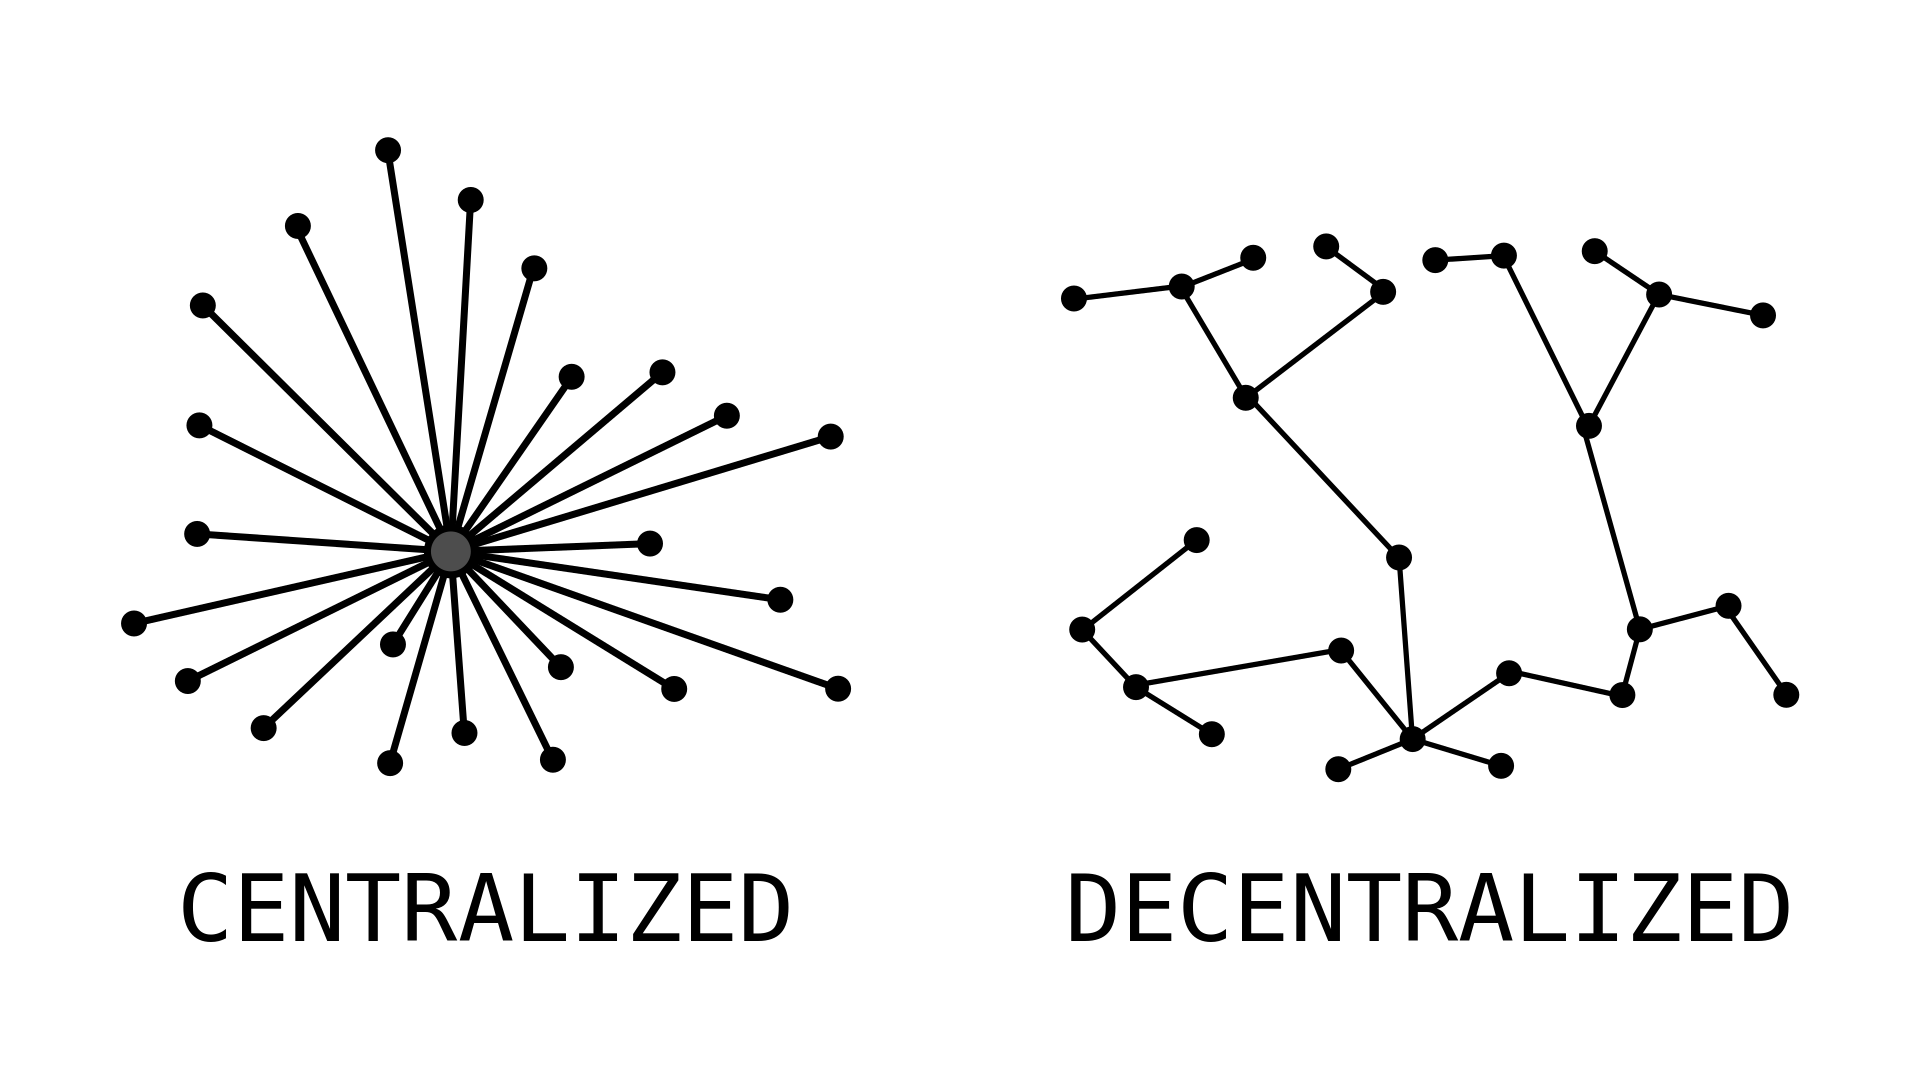
\includegraphics[width=0.7\textwidth]{Figures/Decentralization_diagram.png}
    \caption{Digrama explicando la descentralización}
    \label{fg:decentralization_diagram}
\end{figure}
Las criptomonedas, permiten liberarnos de los intermediarios. Consiguen que las transacciones se realicen entre dos personas sin necesidad de transmitir esa información por multiples canales para conseguir realizarla.
\subsection{Ethereum}
Ethereum, es la evolución natural de Bitcoin. En su propio whitepaper, hablan de como bitcoin es un estado de transición. Justificando que ethereum, tiene mas bloques de construcción para permitir crear un internet descentralizado. Ethereum aporta cambios sustanciales a la forma en la que es minado y crea un nuevo concepto llamado smart contracts, que permiten la ejecución de código automática en respuesta a eventos que ocurren en la red.
Todos los eventos, son tratados como mensajes. Es un termino parecido a las “transacciones” clásicas en bitcoin. Estos mensajes, no son simplemente envíos de dinero, ya que pueden ser verdaderos mensajes enviados por smart contracts los cuales pueden responder. Haciendo a niveles prácticos una función a la que podemos llamar.
Una transacción, en ethereum tiene las siguientes partes:
\begin{center}
    \begin{table}[h!]
        \begin{tabular}{|p{0.3\linewidth} | p{0.6\linewidth}|}
            \hline
            Mensaje & Mensaje que quiere ser enviado \\
            \hline
            Firma   & Prueba criptográfica que verifica que el sender es quien dice ser. \\
            \hline
            Atributos especiales & \\
            \hline
            STARTGAS &  Para evitar la ejecución de un bucle infinito en el minero, se impone un limite de gas que se va quemando mientras la ejecución avanza. Cuanto mas se tarde en ejecutar mas gas se quema. \\
            \hline
            GASPRICE & Por cada unidad de gas que es quemada, se le pagará al minero con su equivalencia en ether. \\
            \hline
        \end{tabular}
        \label{tab:ethereum_msg}
        \caption{Tabla explicando el desglose de un mensaje de ethereum.}
    \end{table}
\end{center}
Gracias a estos atributos especiales, podemos generar una experiencia de usuario mejor.
\begin{itemize}
    \item Si alguna transacción llegase a fallar, se le devolvería el gas restante. Estos fallos, se pueden tirar con \texttt{require}. Esta keyword reservada espera un booleano con evaluación positiva.
Este código muestra \texttt{require} es funcionamiento.
\begin{lstlisting}
    function foo()
    public
    {
    // ... 
    // La ejecucion continua
    require(true,
    'Mensaje para enviar al sender si llega a fallar');
    // Si algun check llega a fallar se revierte el estado 
    require(false,
    'El sender vera este mensaje ya que el booleano es falso');
    // ...
    }
\end{lstlisting}
    \item Si alguna transacción se queda sin gas, el estado se revierte al inicial pero el dinero es perdido.
\end{itemize}

\subsection{Minería}
La minería es el concepto de verificar las transacciones que ocurren en la red. A día de publicación de este trabajo, el sistema de verificación que utiliza es proof-of-work. Al utilizar el mismo mecanismo de protección, sus transacciones se parecen.
\begin{figure}[h!]
    \centering
    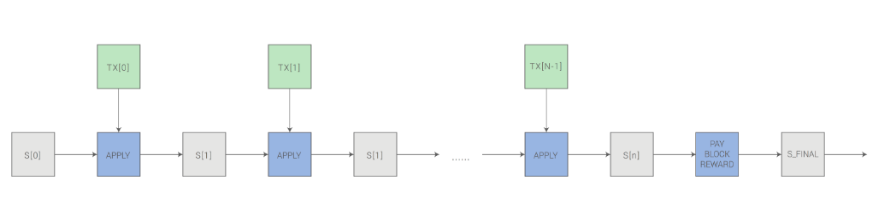
\includegraphics[width=0.8\textwidth]{Figures/Screenshot_20220507_131504.png}
    \caption{Diagrama que explica la mineria}
    \label{fg:block_diagram}
\end{figure}
La red de ethereum, siempre se asegura que se genera un bloque cada 12 segundos.
Estos 12 segundos son una especie de latido que muestra la salud de la red de ethereum. Para mantener siempre ese ritmo, se ajusta la dificultad de minado.
\begin{enumerate}
    \item Se genera una transacción y se firma con la clave privada.
    \item El usuario comparte la petición a toda la red de ethereum desde un minero.
    \item En algún momento de esos 12 segundos, un minero puede llegar a agregar cientos de transacciones en un posible bloque, en una manera que maximiza las comisiones de transacción. Todo esto mientras están por debajo del limite de gas.
    \begin{enumerate}
        \item Verifica la legitimidad de la transacción. i.e la firma corresponde al mensaje y si la cuenta tiene liquidez.
        \item Inicia el proceso de proof of work. Este proceso se basa en los siguientes parámetros. Dificultad del bloque ex. \texttt{3,324,092,183,262,715}, mixHash ex.\\ \texttt{0x44bca881b07a6a09f83b130798072441705d9a665c5ac8bdf2f39a3cdf3bee29} y la sal (numero hexadecimal aleatorio) \texttt{0xd3ee432b4fb3d26b}. Proof of work es una carrera entre todos los mineros de la red para ver quien puede generar. Cuando se genera un hash con SHA 256 ex. \\\texttt{ba7816bf8f01cfea414140de5dae2223b00361a396177a9cb410ff61f20015ad} se busca que un hash con una cierta cantidad de ceros al principio. La dificultad del bloque es cuantos hashes se pueden ser correctos para ese bloque. Cuanto menor sea el numero mas difícil es verificar ese bloque.
    \end{enumerate}
    \item Eventualmente, algún minero conseguirá solucionar el puzzle criptográfico y nuestro mensaje estará aceptado en la blockchain. Ese bloque contiene el checksum de todas los elementos internos.
    \item El resto de la red, al escuchar que un minero ha conseguido solucionar el bloque, lo verifica y si es correcto lo toma como el estado canónico de la red.
    \item Por ultimo los mineros borran de su memoria la lista de su mempool.
\end{enumerate}
\textbf{Limitaciones}\\
Proof-of-work, como se ha explicado, es una operación computacionalmente intensa. En una red congestionada como esta en estos momentos, la dificultad de los bloques esta explotada. Aún así, el consumo energético, comparando con Bitcoin famosas, es inferior \ref{fg:consumo}.
\begin{figure}[h!]
    \centering
    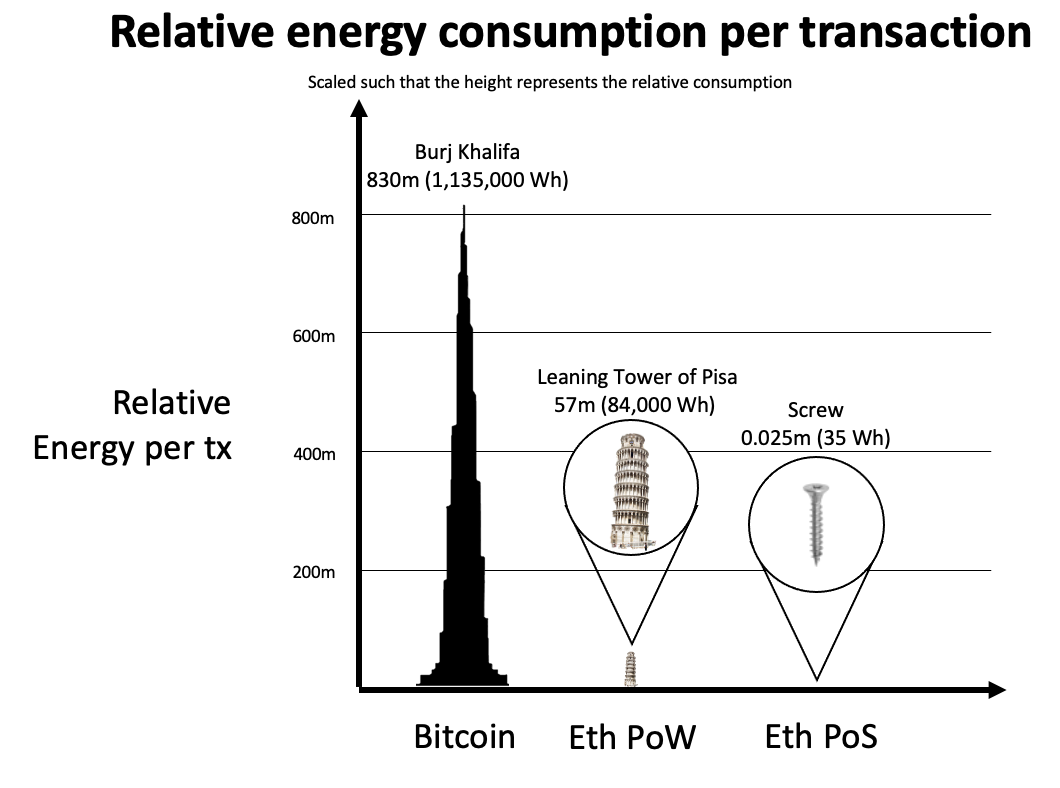
\includegraphics[width=0.6\textwidth]{Figures/consumo.png}
    \caption{Diagrama comparativo de consumo energético por transacción}
    \label{fg:consumo}
    \cite{web:eth_energy}
\end{figure}
Aú así, Esto hace que si tenemos aproximadamente 70 transacciones en un bloque, estamos gastando 5880000 Wh.
Ethereum quiere actualizar su método de verificación a proof-of-stake. Esto cambiaría a un modo de verificación computacionalmente caro a otro que no lo es tanto. Antes que ese cambio ocurra, Ethereum seguirá consumiendo en un año lo mismo que Finlandia y tiene una huella de carbono comparable a Bulgaria \cite{web:carbono}.
A fecha de publicación de este proyecto, Ethereum 2.0 no está implementado. Se lleva desde 2016 una bomba de dificultad para migrar a los usuarios pero esa bomba todavía \textit{no ha explotado}. Esta bomba existe para evitar que se cree una copia. Esa bomba hará que la dificultad carezca de manera exponencial hasta que minar un nuevo bloque sea imposible. Se lleva retrasando año tras año. Se ha retrasado un total de 5 veces. Por ahora tiene fecha de junio de 2022. Aún así, en el EIP-4345 \cite{web:eip_bomb}, se da la posibilidad de atrasarlo más.
Hasta que no se haga el cambio de algoritmo de verificación, Ethereum seguirá contaminando. Esta implicación ética, se investigará un el apartado correspondiente.
\subsection{Gas}
Como se ha explicado antes, se puede ejecutar código en la red de ethereum. Para proteger la red, existe una pequeña tarifa que hay que pagar por cada momento de ejecución. Así se evitan la existencia de ataques por parte de actores malignos.
Cuando una transacción se completa, se envía de vuelta el gas resultante al origen \ref{fg:message_diagram}.
\begin{figure}[h!]
    \centering
    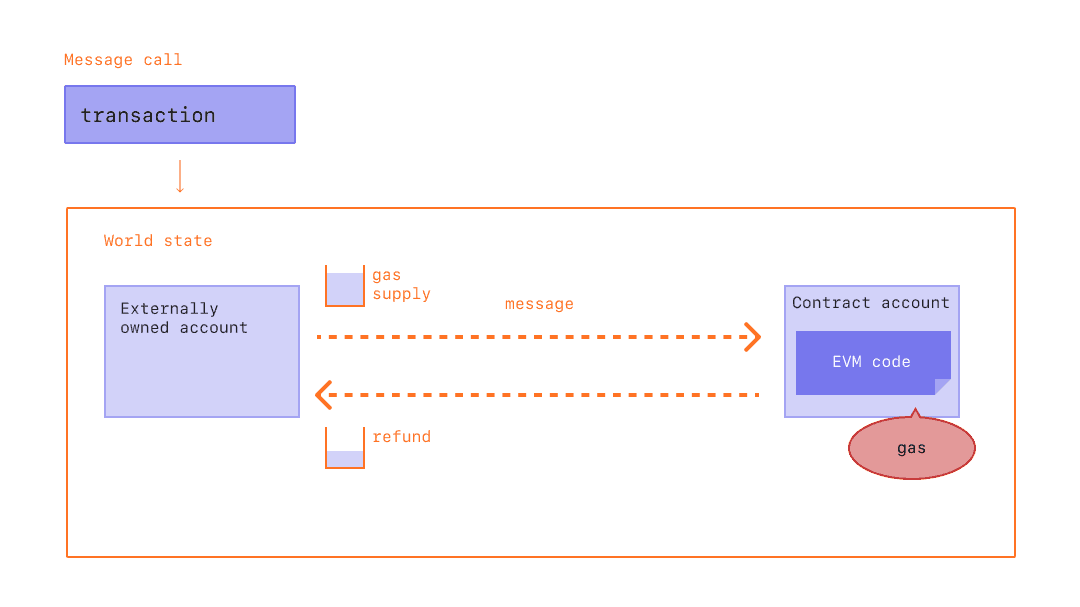
\includegraphics[width=0.8\textwidth]{Figures/gas-tx.png}
    \caption{Diagrama que explica el uso de gas}
    \label{fg:message_diagram}
\end{figure}
\begin{equation}
    max fee - (base fee + tip) = refund
\end{equation}
Después de la “London update”, el gas en ethereum ha evolucionado para proteger mas a los usuarios de posibles manipulaciones por parte de los mineros.
\subsection{Smart Contracts}
Un smart contract, es un programa que vive en la blockchain. A niveles prácticos, un contrato es como si fuese otra persona de la red con la que interactuamos.
Si nosotros tenemos la dirección
\say{0xc0ffee254729296a45a3885639AC7E10F9d54979}
un contrato puede tener la dirección
\say{0x70E3Aed5aA1aac6EC39D114B7411DF6f1CC80671}
Todos los mensajes compartidos entre los usuarios y un smart contract quedan grabados para siempre en la cadena de bloques global. Como se ha dicho anteriormente, en ethereum las transacciones se llaman mensajes, porque su contenido no es simplemente dinero, puede tener una infinidad de funciones.
Los smart contracts, una vez creados no pueden ser destruidos, para ser actualizado por ejemplo, requeriría hacer deploy de nuevo.
\begin{lstlisting}
    pragma solidity 0.8.7;

    contract VendingMachine {
    
        // Declare state variables of the contract
        address public owner;
        mapping (address => uint) public cupcakeBalances;
    
        // When 'VendingMachine' contract is deployed:
        // 1. set the deploying address as the owner of the contract
        // 2. set the deployed smart contract's cupcake balance to 100
        constructor() {
            owner = msg.sender;
            cupcakeBalances[address(this)] = 100;
        }
    
        // Allow the owner to increase the smart contract's 
        // cupcake balance
        function refill(uint amount) public {
            require(msg.sender == owner, "Only the owner can refill.");
            cupcakeBalances[address(this)] += amount;
        }
    
        // Allow anyone to purchase cupcakes
        function purchase(uint amount) public payable {
            require(msg.value >= amount * 1 ether, 
            "You must pay at least 1 ETH per cupcake");
            require(cupcakeBalances[address(this)] >= amount,
            "Not enough cupcakes in stock to complete this purchase");
            cupcakeBalances[address(this)] -= amount;
            cupcakeBalances[msg.sender] += amount;
        }
    }
\end{lstlisting}
Tomando de ejemplo el código de la wiki de ethereum, se va a explicar su funcionamiento. \cite{web:sample_smart_contract}
Solidity, el lenguaje de programación DSL (domain specific language) que utiliza la blockchain Ethereum, tiene un paradigma de programación basado en objetos. Por eso mismo, su sintaxis es similar a los lenguajes C-like, por ejemplo java.
En el siguiente bloque de código, especificamos la version de solidity que vamos a utilizar. En este caso y fecha de publicación de este proyecto la más reciente, \verb|0.8.7|.
\begin{lstlisting}
    pragma solidity 0.8.7;
\end{lstlisting}
Después podemos definir nuestro objeto. Para este ejemplo, vamos a crear una maquina de \textit{vending}.
\begin{lstlisting}
    contract VendingMachine {//...}
\end{lstlisting}
En este lugar, funcionaria de una manera parecida a un programa clásico en java. Las variables de ese objeto se pueden declarar directamente, estableciendo si son públicas o privadas. Ser pública significaría que esa variable es accesible por otros módulos. Permitiendo utilizar su valor o modificarlo directamente.
En nuestra máquina dispensadora, vamos a guardar la dirección de nosotros mismos para poder por ejemplo reponer la maquina. Solidity tiene un tipo nativo que puede guardar direcciones directamente.
\begin{lstlisting}
    address public owner;
\end{lstlisting}
Ahora sólo se necesita llenar la maquina. Esta maquina, es un poco peculiar y solo se venden magdalenas. En este punto, podemos crear un mapa que asocie cantidades a direcciones en especifico.
Si la dirección de nuestro contrato es
\begin{displayquote}
    0x70E3Aed5aA1aac6EC39D114B7411DF6f1CC80671
\end{displayquote}
Podemos hacer que si buscamos el valor asociado a esa dirección sea el contenido de esa dirección obtengamos el balance.
\begin{lstlisting}
    mapping (address => uint) public cupcakeBalances;
\end{lstlisting}
Para poder llenar la maquina nada mas instalarla, existe el constructor. Un método constructor en java, se ejecuta cuando se crea una nueva instancia del objeto con la keyword \verb|new|. En este caso, nuestro constructor es llamado una vez se añade a la blockchain. Por este motivo, nos cuesta gas hacer deploy de un contrato.
\begin{lstlisting}
    // When 'VendingMachine' contract is deployed:
    // 1. set the deploying address as the owner of the contract
    // 2. set the deployed smart contract's cupcake balance to 100
    constructor() {
        owner = msg.sender;
        cupcakeBalances[address(this)] = 100;
    }
\end{lstlisting}
Por último, tenemos las funciones clásicas. En una maquina solo se puede añadir elementos y que alguien los compre. Estas, se pueden crear con la keyword \verb|function|. Estas funciones, pueden comportarse como voids o como una persona a la que pagar con \verb|payable|.
Gracias a \verb|require|, podemos crear puntos de control, que por ejemplo permitan que solo el creador pueda añadir más magdalenas a la máquina. No solo eso, sino que podemos asegurarnos que tengan el dinero necesario y que queden magdalenas en la máquina.
\begin{lstlisting}
    // Allow the owner to increase the smart contract's cupcake balance
    function refill(uint amount) public {
        require(msg.sender == owner, "Only the owner can refill.");
        cupcakeBalances[address(this)] += amount;
    }

    // Allow anyone to purchase cupcakes
    function purchase(uint amount) public payable {
        require(msg.value >= amount * 1 ether, 
        "You must pay at least 1 ETH per cupcake");
        require(cupcakeBalances[address(this)] >= amount, 
        "Not enough cupcakes in stock to complete this purchase");
        cupcakeBalances[address(this)] -= amount;
        cupcakeBalances[msg.sender] += amount;
    }
\end{lstlisting}
\textbf{Limitaciones}\\
La gran limitación de los smart contracts, es la inmutabilidad de la red. Una vez se publica ese contrato, no se puede actualizar. Si se descubre un fallo o se quiere cambiar la lógica se necesita volver a publicar el contrato. Esto implica que no solo el contrato sigue existiendo para siempre, sino que hay que direccionar a nuestros usuarios a el nuevo contrato.
Como se explicará mas adelante, esto supone que hay que cambiar la dirección que le aportamos a los usuarios a través de nuestro \textit{payload} de js.
\subsection{Puntos débiles de la solución elegida}
Antes de la \textit{London Update}, los mineros podían llegar a manipular el precio ralentizando la ejecución y usando todo el gas del usuario. Esto suponía que los usuarios que quisieran hacer una transacción, se encontraban con la necesidad de llenar con mas gas su transacción para que algún minero la ejecutase en un tiempo aceptable. El resto de usuarios, si querían que su transacción no tardase 30 minutos como mínimo, tendría que inevitablemente pagar más.
Para evitar eso, se introdujo un limite de gas en cada bloque. Ademas, los usuarios podían poner un rango de gas que estarían dispuestos a pagar. De esta forma, se busca que los bloques sean lo mas eficientes posibles.
Actualmente, tanto la dificultad de los bloques y como el gas medio de transacción esta disparado\cite{web:gas_price}. Esto hace que cualquier transacción tenga un coste añadido. Moderadores de r/ethereum, dicen lo siguiente cuando son preguntados sobre si el alto precio del gas \textit{matará} ethereum.
\begin{displayquote}
    \textbf{High gas fees will kill Ethereum}\\
    This is one of those bizarre comments that pervades through crypto retail doesn't seem to make any sense. Overwhelming demand for a product will somehow... kill a project? It's like saying AMD and Nvidia are going to die soon because graphics cards are now grotesquely overpriced.
    No, the reality, like I said above, is that there's overwhelming demand for EVM blockspace and a limited supply of gas. Currently, the high fees shows there's incredible demand for Ethereum L1 blockspace, and people are willing to pay a steep premium for it.
    This is what gives the Ethereum network and ETH value. And in two months' time, there'll be a mechanism with EIP-1559 to accrue this value to every ETH stakeholder.
    Over time, we will see gas fees drop with a greater supply of gas - the reality is that there'll never quite be enough blockspace supply to satisfy global demand for EVM blockspace long term. There'll be rollups, there'll be hybrid solutions like zkPorter/Validium, there'll be sidechains/alternate chains, and there'll be centralized solutions. The ecosystem will work together to offer different trade-offs with decentralization versus transaction fees.
    \cite{web:reddit_ethereum}
\end{displayquote}
Aunque queda mucha discusión en comentarios.
\begin{displayquote}
    Your answer for fees is far from being satisfying. Yes high fees will kill Eth. Your Nvidia example isn't the same thing.
    You know there are other successful blockchains coming strong. Avalanche for one has lots of Dapps on it. People will quit using Eth at some point if this doesn't change. Because other chains have already solved that problem...
    And I wouldn't care about any supply problem for a global demand, because this won't be an issue. We all use Eth because we have to and we all know it.
    \cite{web:reddit_ethereum_comment}
\end{displayquote}
Es un problema que los contribuidores de ethereum tendrán que combatir y probar en una de las redes más grande del mundo. Como Ethereum es código abierto, se pueden crear \textit{Ethereum Improvement Proposals} - EIP\cite{web:EIP}. Es una manera de la que la comunidad puede mejorar y actualizar la red.
\section{Introducción a envíos de datos a través de un medio distribuido}
\begin{displayquote}
    IPFS \cite{web:ipfs} is a distributed system for storing and accessing files, websites, applications, and data. \cite{web:ipfs_whatis}
\end{displayquote}
IPFS \cite{web:ipfs}, es una red descentralizada que permite compartir datos de manera muy sencilla. IPFS \cite{web:ipfs} consigue tener una mayor distribución del ancho de banda.
Todos los nodos de la red pueden esta conectados entre si teniendo una interconexión eficiente. Los ficheros subidos a IPFS \cite{web:ipfs} tienen un CID (Content IDentifier). Ese CID es un registro permanente de la existencia de ese fichero como existe en el tiempo.
Cuando otro usuario busca tu CID \ref{fg:looking_for_CID}, pregunta al resto de los usuarios donde esta el fichero. Cuando lo reciben, lo cachean y se convierten en proveedores de tu fichero.
\begin{figure}[h!]
    \centering
    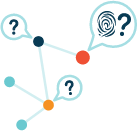
\includegraphics[width=0.2\textwidth]{Figures/svgviewer-png-output.png}
    \caption{Diagrama que explica la busqueda de un CID}
    \label{fg:looking_for_CID}
\end{figure}
Un usuario, puede anclar (pin) un fichero para guardar y proveer tu fichero para siempre. En cambio, los contenidos que no tengan ese pin serán descartados para liberar memoria. Esto significa que los usuarios solo guardan lo en lo que están interesados, mas un pequeño indice para saber que usuario tiene que.
Todos los ficheros van acompañados de un hash, haciendo que si alguien intenta cambiar el fichero o sus datos, resultara en un cambio en el hash. Esto implica que se le asignara un CID distinto. Esto significa que nuestros ficheros una vez subidos están seguros y serán resistentes ante la censura y la manipulación \ref{fg:keeping_IPFS_safe}.
En la siguiente sucesion de figuras, ponemos a prueba los pasos para iniciar una conexion.
\begin{center}
\begin{figure}[h!]
    \centering
    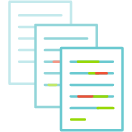
\includegraphics[width=0.2\textwidth]{Figures/svgviewer-png-output(2).png}
    \caption{Diagrama que explica la protección ante censura}
    \label{fg:keeping_IPFS_safe}
\end{figure}
\end{center}
\subsection{Servidores Star}
Para que los nodos se puedan conocer, primero necesitan contactar con algún nodo conocido.
Para encontrar a alguien, tienen las siguientes opciones.
\begin{enumerate}
    \item Tablas de hashing distribuidas.
    \item Paquetes broadcast en la red local.
    \item Compartir listas de peers con peers conocidos.
    \item Trackers o puntos de encuentro centralizados.
    \item Lista de servidores star
\end{enumerate}
Los servidores son muy útiles ya que te devuelven información de donde están tus peers mas cercanos con los que poder empezar a compartir.
Para comprender mejor la situación, vamos a ver unas figuras.
\begin{itemize}
    \item Tenemos un servidor Star que tiene metadatos de los peers que están cerca.
    \item Las lineas grises son conexiones pasadas que han dejado el rastro del handshake. REFACTOR
    \item Las lineas negras son conexiones activas de IPFS \cite{web:ipfs} (libp2p).
    \item La figura verde quiere entrar a la red.
\end{itemize}
\begin{figure}[h!]
    \centering
    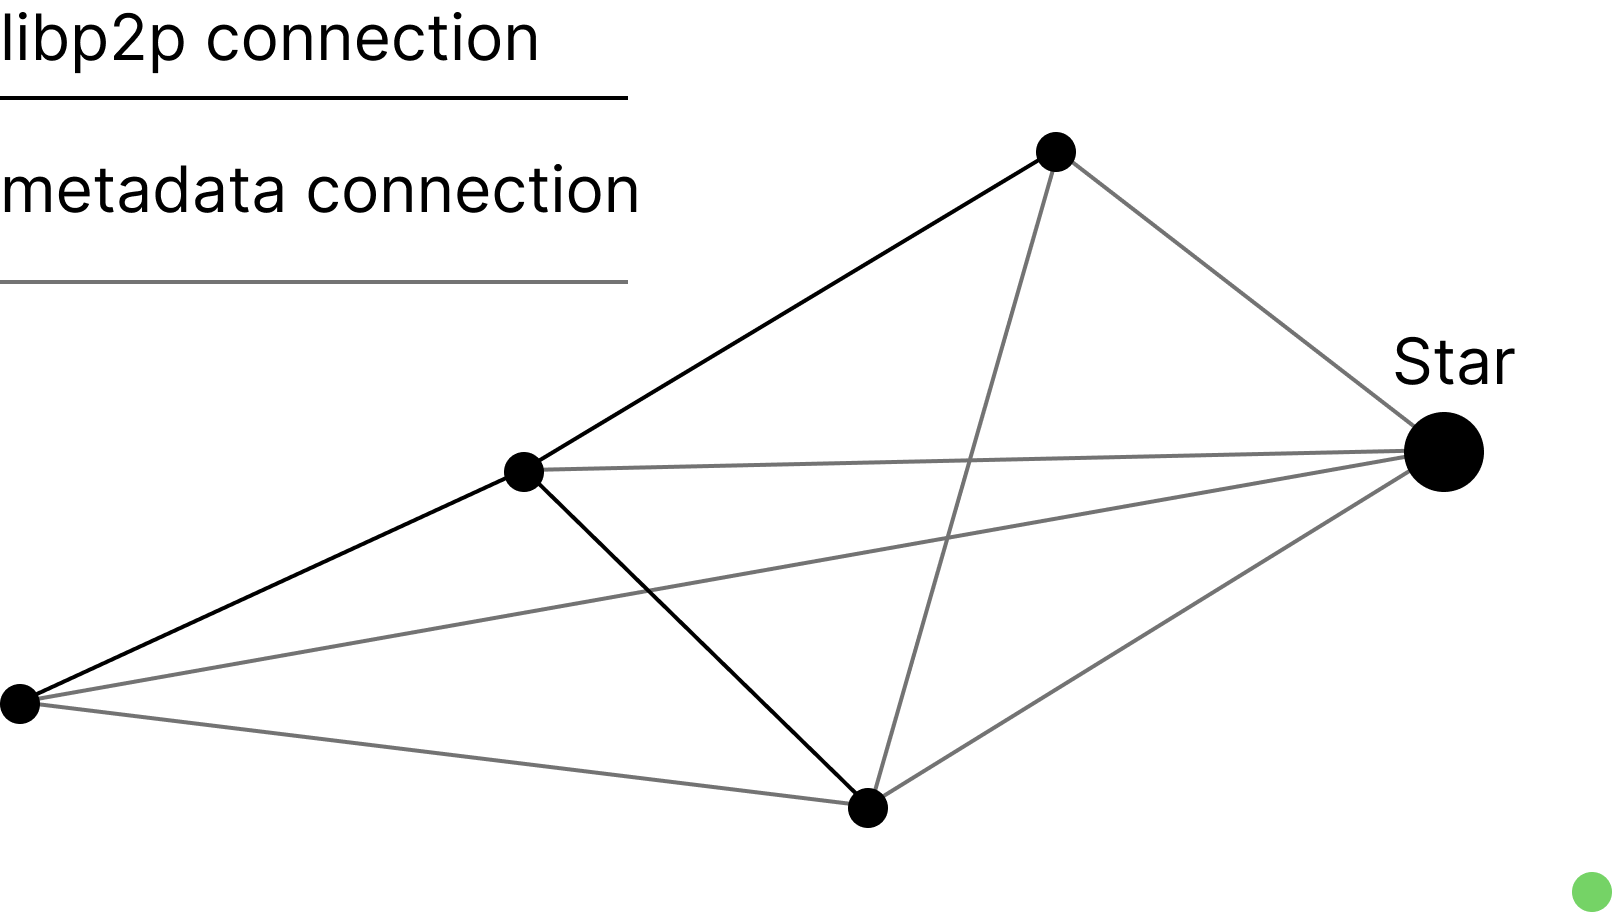
\includegraphics[width=0.7\textwidth]{Figures/Green wants to join(2).png}
    \caption{Diagrama en el que el nodo verde quiere entrar en la red IPFS \cite{web:ipfs}}
    \label{fg:scanning_ipfs}
\end{figure}
\begin{figure}[h!]
    \centering
    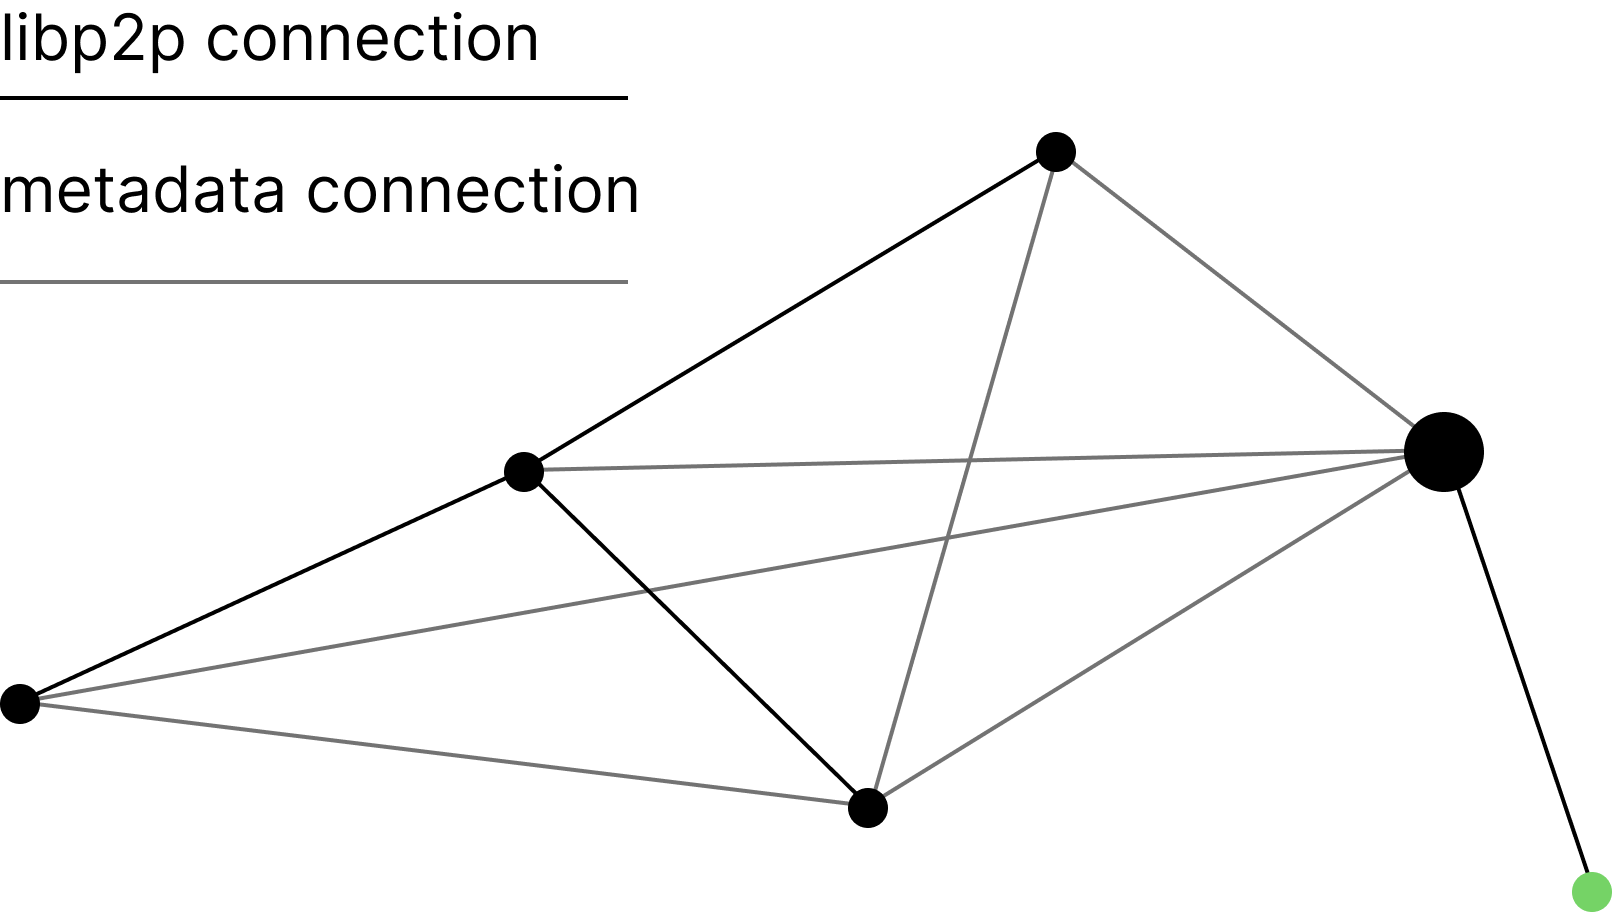
\includegraphics[width=0.7\textwidth]{Figures/Green ask Star for instructions.png}
    \caption{Diagrama en el que el nodo verde pregunta a Star donde estan el resto de las personas}
    \label{fg:asking_star}
\end{figure}
\begin{figure}[h!]
    \centering
    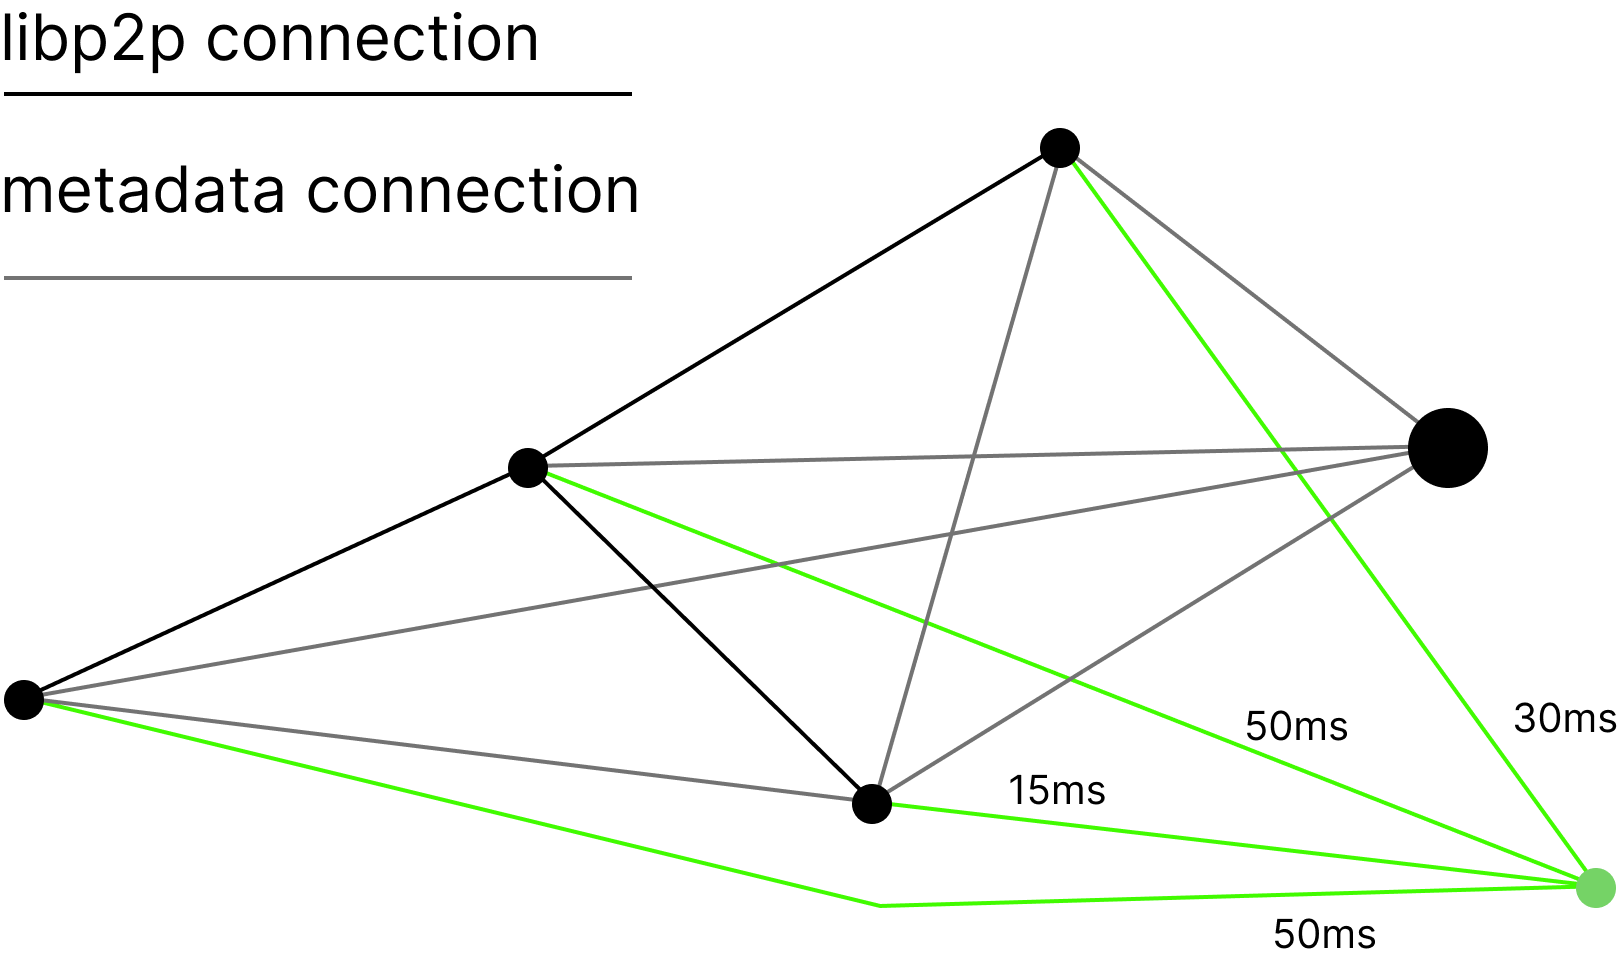
\includegraphics[width=0.7\textwidth]{Figures/Green scans the other peers.png}
    \caption{Diagrama en el que el nodo verde escanea sus alrededores para ver que conexion es mas eficiente}
    \label{fg:scanning_area}
\end{figure}
\begin{figure}[h!]
    \centering
    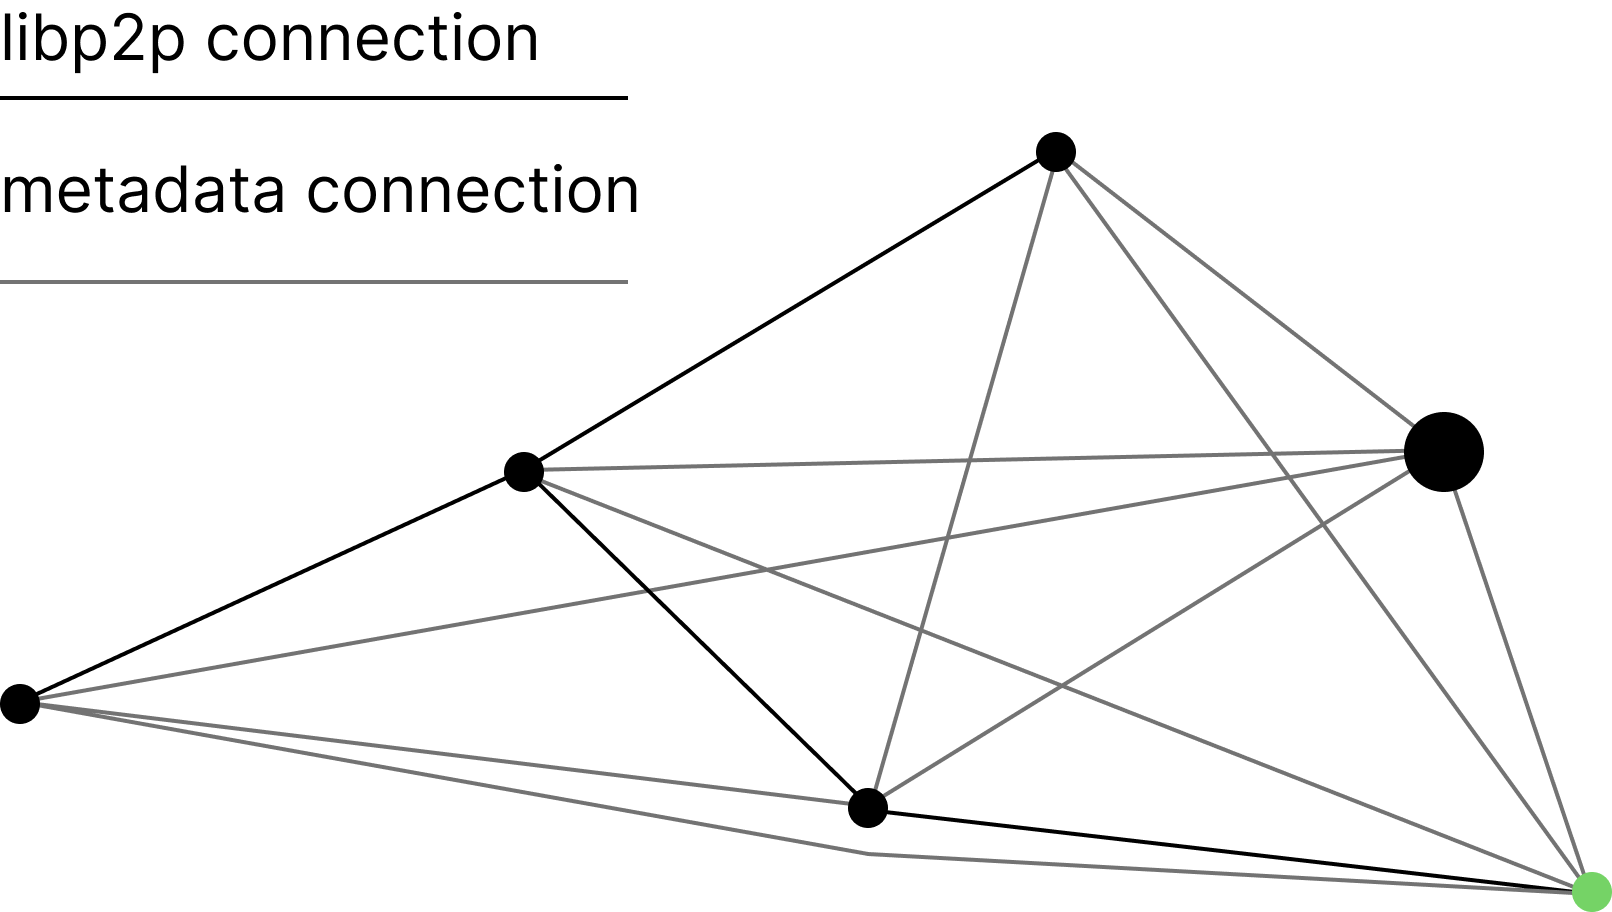
\includegraphics[width=0.7\textwidth]{Figures/Green finally joins(1).png}
    \caption{Diagrama en el que el nodo verde finalmente se conecta}
    \label{fg:connecting}
\end{figure}
\subsection{Nodos y relés}
Los nodos, son los usuarios a los que se hacia referencia anteriormente. Estos nodos pueden ser desde usuarios verídicos ejecutando js-ipfs \cite{web:js-ipfs} en su navegador, o una instancia de go-ipfs o js-ipfs \cite{web:js-ipfs} en un servidor para garantizar nodos de alta velocidad.

Estos nodos tienen un repositorio en el que guardan fragmentos de datos que están alojando o bien que han pasado por el y ha cacheado.

Otra función principal de un nodo es retransmitir información. Para realizar esta función, tienen que estar conectados a otros nodos de la manera que hemos visto en el punto anterior.
\begin{figure}[h!]
    \centering
    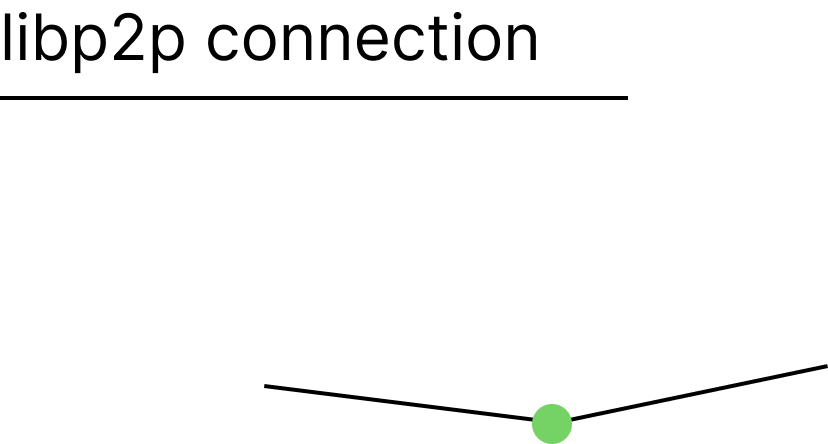
\includegraphics[width=0.4\textwidth]{Figures/Angulo 2.png}
    \caption{El nodo de color verde tiene un nivel de red 2. Ya que hay dos conexiones activas.}
    \label{fg:network_dgr}
\end{figure}
Primero vamos a ver el concepto de nivel de red. Las opciones predeterminadas de libp2p para el nivel ideal es \verb|6|. Un nivel entre \verb|4| - \verb|12| es un nivel \textit{aceptable}.
\begin{quote}
    Por simplicidad en los diagramas el Lower bound = 2 y el Upper bound = 4.
\end{quote}
Viendo esto, necesitamos un modo inteligente en el que asegurar que todos los nodos reciben la información sin duplicidades.
\begin{figure}[h!]
        \centering
        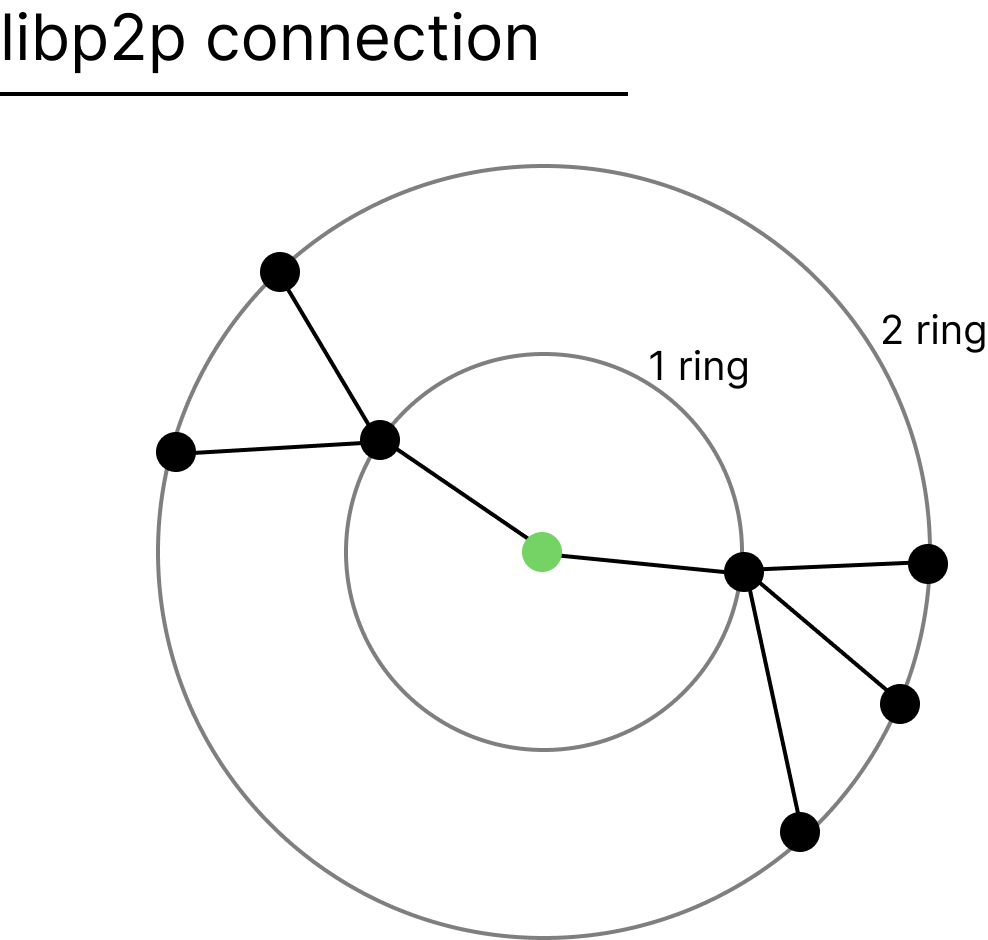
\includegraphics[width=0.5\textwidth]{Figures/Radios de comunicacion.png}
        \caption{Mapa de conexiones desde el punto de vista del nodo verde. \textbf{La conexión de metadatos ha sido omitida por razones de claridad.}}
        \label{fg:Mapa_de_conexiones}
\end{figure}
Si un dato del ring 2 quiere llegar hasta el nodo verde, aparentemente, al no tener una conexión directa no podría hacerlo, pero como los nodos actúan de \textit{relays}, los datos pueden pasar por el ring 1 hasta llegar al nodo verde.
Al hacerlo, los nodos que viven en el ring 1, si los datos han pasado por ellos, pueden guardar esos datos para que si el nodo verde las vuelve a solicitar, se le envíen con menor latencia.
Aplicando pruning, el grafo anterior, quedaría de la siguiente manera \ref{fg:mapa_optimizado}.
\begin{figure}[h!]
    \centering
    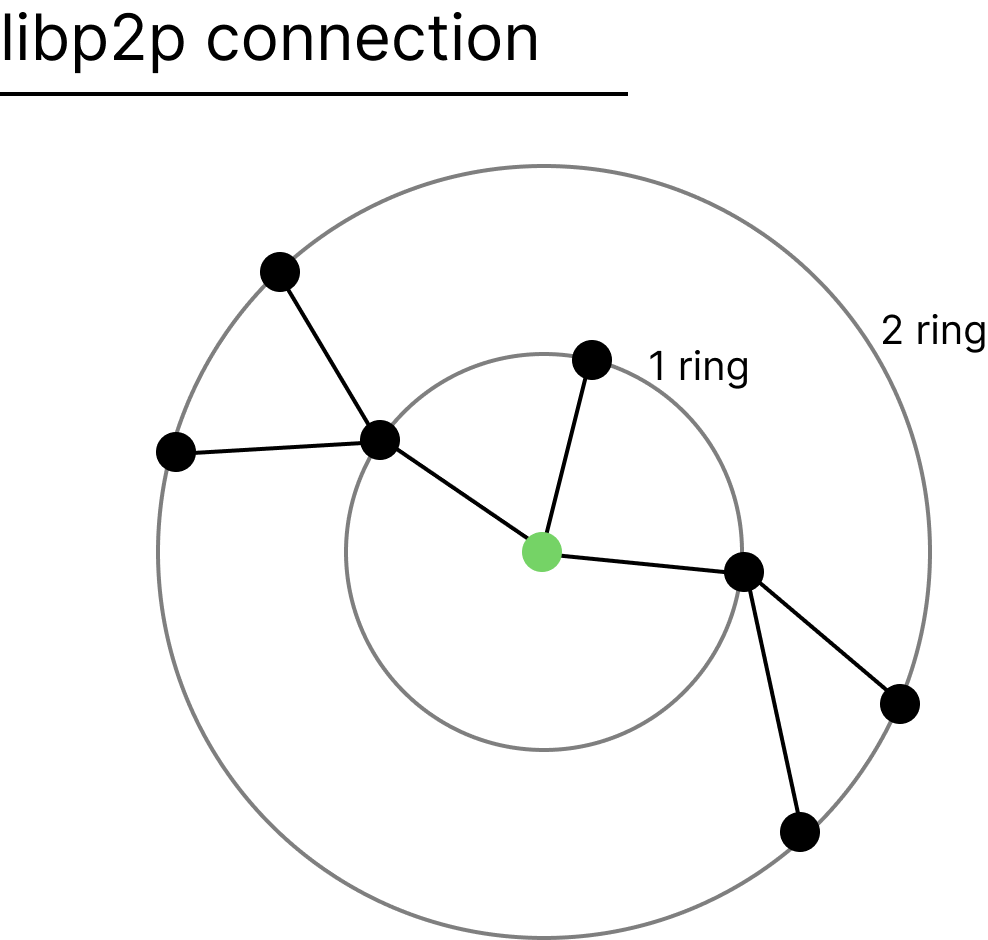
\includegraphics[width=0.5\textwidth]{Figures/Radios de comunicacion optimizado.png}
    \caption[El nodo verde optimiza la conexión]{El nodo verde optimiza la conexión. \textbf{El nodo movido, también calcularía cual seria su conexión optima, pero todas las conexiones se ven desde el punto de vista del nodo verde.}}
    \label{fg:mapa_optimizado}
\end{figure}
Esto significa que como el nivel de conexión optimo es 3, en la figura original \ref{fg:Mapa_de_conexiones} la red no es optima. Nuestro nodo verde tiene 2 y el nodo en la parte inferior derecha tiene 4. Para poder generar un grafo más óptimo, el nodo verde tendria que tener 3 conexiones y el nodo en la parte inferior derecha también. Por eso mismo nuestro nodo verde inicia una nueva conexión óptima y el nodo en la parte inferior derecha borra una conexión, resultando en \ref{fg:mapa_optimizado}.
\subsection{Pub Sub}
Pub Sub \ref{fg:pubSub}, es una parte del spec de IPFS \cite{web:ipfs}, el cual es fundamental para el funcionamiento.
\begin{figure}[h!]
    \centering
    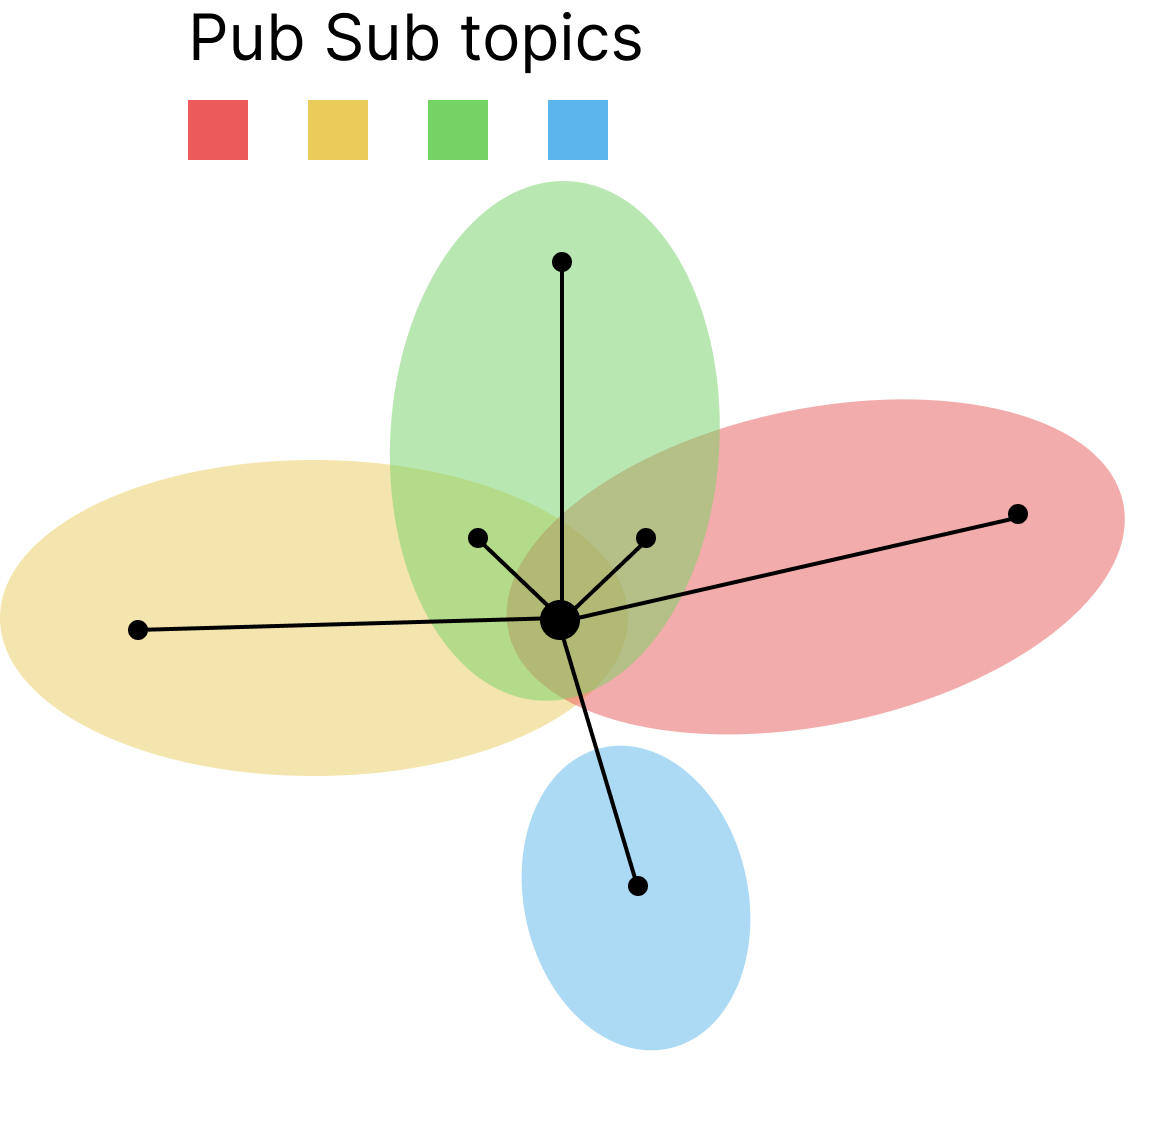
\includegraphics[width=0.7\textwidth]{Figures/Pub Sub.png}
    \caption{Diagrama explicando el funcionamiento de pub sub. Punto de vista del nodo central.}
    \label{fg:pubSub}
\end{figure}
Pub Sub, permite subscribirse a un topic. Un topic se define como un \verb|string|.
Pongamos como ejemplo que existen los siguientes topics.
\begin{itemize}
    \item \verb|Rojo|
    \item \verb|Verde|
    \item \verb|Amarillo|
    \item \verb|Azul|
\end{itemize}
El host central, esta subscrito a los topics \verb|Amarillo|, \verb|Verde| y \verb|Rojo|.  Aun así, como el nodo central esta conectado a un nodo solo subscrito a un topic \verb|Azul|. Esto se debe ya que libp2p intentara mantener una conexión saludable. Nuestro nodo no está sólo interesado en escuchar a su topic, sino ayudar establecer una red saludable en la que hacer llegar la información necesaria a todos los nodos interesados.
\begin{figure}[h!]
    \centering
    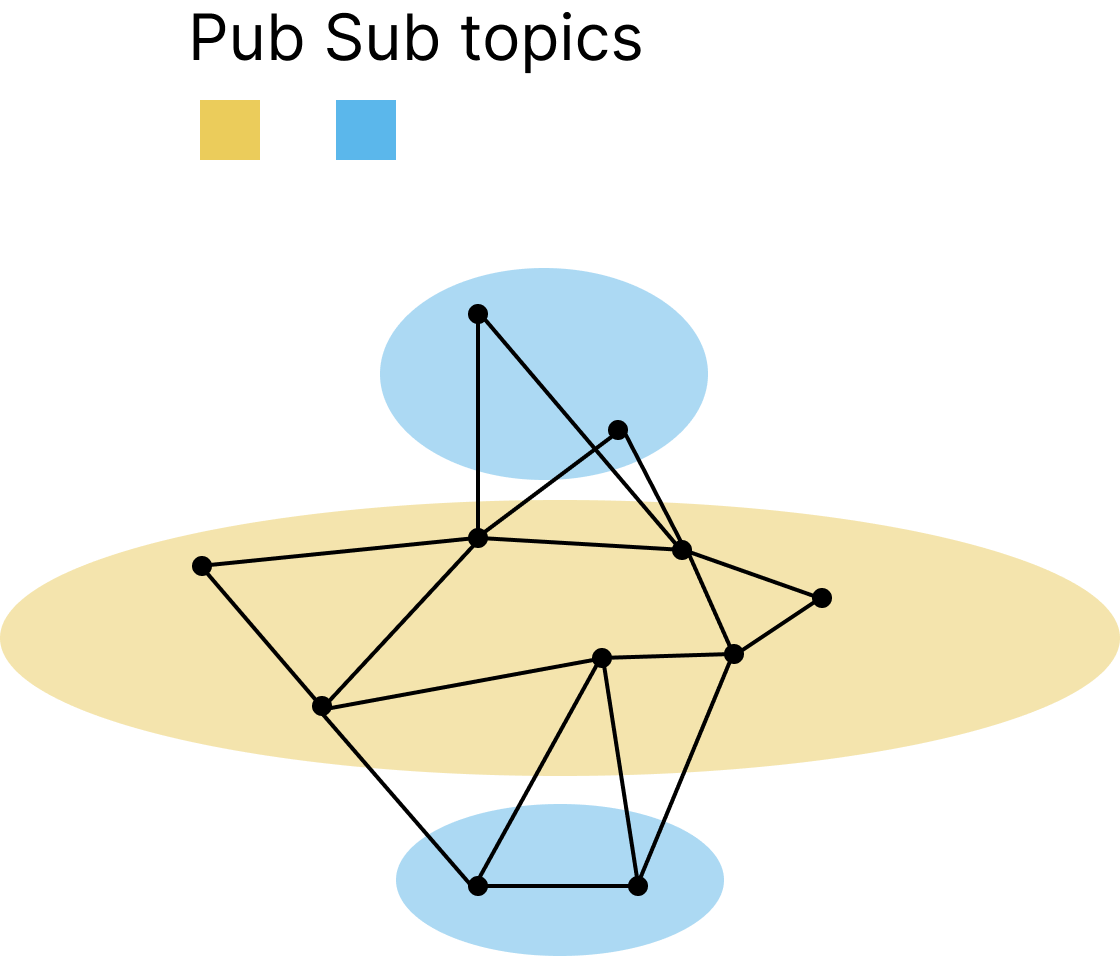
\includegraphics[width=0.7\textwidth]{Figures/Zonas multiples.png}
    \caption{Grafo de ejemplo para explicar la donación de temas.}
    \label{fg:zonas_multiples}
\end{figure}
En este posible grafo de conexión \ref{fg:zonas_multiples}, hay 4 hosts que están subscritos a el tema \verb|Azul|. Si los host que están escuchando al topic \verb|Amarillo|, no pasasen el mensaje, las dos zonas azules no estarían comunicadas.
Como los nodos comparten todos los mensajes y guardan metadatos de los mensajes que pasar por ellos. Por eso, los nodos que escuchan al tema amarillo, pueden hacer de relés y pasar todos los mensajes.
De este modo, IPFS \cite{web:ipfs} nos permite crear una red global de envío de mensajes instantáneos de manera gratuita y con un sistema resistente a fallos, ya que nuestros paquetes tienen varias rutas por las que ir y reparten carga entre las rutas posibles.
\subsection{Alternativas}
A la hora de compartir información de manera distribuida, hay muchas opciones. Una de ellas, también muy popular en el presente, es webtorrent \cite{web:webtorrent}. Un librería que trae las tecnologías torrent a la web.
Este proyecto, utiliza webrtc, lo mismo que IPFS \cite{web:ipfs} para conseguir la funcionalidad. webrtc, no se usa en el resto de la red. Significando que existe una ruptura en la red. Aunque los dos se basen en un archivo \verb|.torrent| muy parecido a lo que implica que sino tienes peers compartiendo esa información utilizando un cliente compatible no puedes acceder a el.
\begin{figure}[h!]
    \centering
    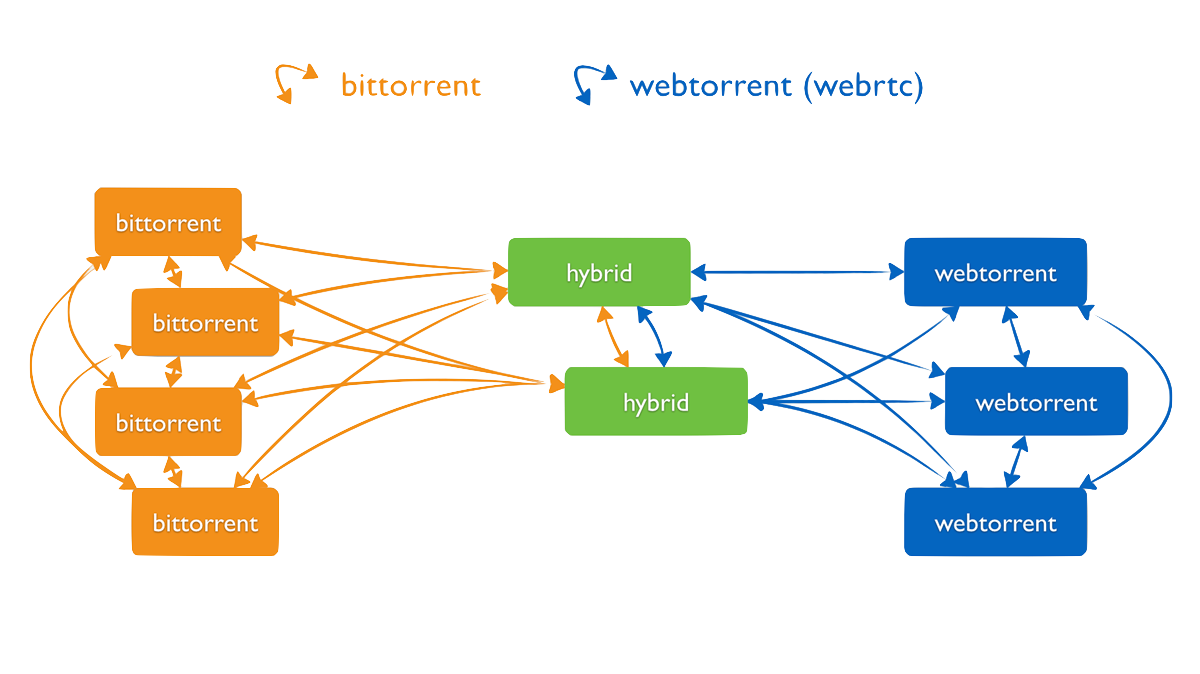
\includegraphics[width=0.6\textwidth]{Figures/68747470733a2f2f776562746f7272656e742e696f2f696d672f6e6574776f726b2e706e67.png}
    \label{fg:webtorrent}
\end{figure}
En la web, dan las herramientas a desarrolladores de programas torrent a implementar un adaptador entre las dos redes. Por ahora solo \textbf{WebTorrent Desktop, Vuze, webtorrent-hybrid, Playback, instant.io y \(\beta\)Torrent} han implementado un adaptador. Convirtiéndose en un nodo \textbf{\textit{hybrid}}.\\
% TODO: Explorar wormhole %
\textbf{Desventajas de utilizar webtorrent}\\
Como ya se ha comentado hay una division en la red, llevando a una división y en definitiva falta de nodos, con todos los beneficios que nos trae el tener muchos.
Otra gran desventaja, es la \textbf{inmutabilidad}.
\begin{quote}
    \textbf{Is it possible to do live streaming with WebTorrent?}\\
    WebTorrent cannot do live streaming out-of-the-box, however you can build a live streaming solution on top of WebTorrent.
    Torrents are immutable. That means that once a torrent file is created, it cannot be changed without changing the info hash. So, how could one get around this limitation?
    A naive approach would be this: The content producer could take every 10 seconds of live content and create a torrent for it. Viewers would follow this \textit{feed} of torrent files (or info hashes) and download the content sequentially. Streamers would be around 10-20 seconds behind the live stream.
    This approach can definitely be improved, though! Why not give that a shot yourself and share the code? \cite{web:webtorrent_faq}
\end{quote}
IPFS \cite{web:ipfs}, aunque también sea inmutable por naturaleza para protegerse de censura y manipulación, implementa PUBSUB, una manera de poder implementar cambios en la red. 
Esto hace que en el archivo que reside en el DID solo exista el topic y la identidad de esa persona. Como la base de datos es solo de esa persona, solo esa persona puede añadir identidades ( o retirarlas ). Eso hace que las personas que estén escuchando al topic de IPFS \cite{web:ipfs} también puedan comprobar.
\newpage
\section{Introducción a la criptografía}
Este trabajo requiere criptografía para poder garantizar la seguridad de los datos compartidos. Como hemos visto los datos compartidos en IPFS \cite{web:ipfs}, por cualquier nodo que pasan, son cacheados para permitir una baja latencia en futuros accesos. Esto es un problema, ya que de manera predeterminada IPFS \cite{web:ipfs} no incorpora encriptado de contenido.
\begin{quote}
    \textbf{IPFS \cite{web:ipfs} docs}
    As a protocol for peer-to-peer data storage and delivery, IPFS \cite{web:ipfs} is a public network: Nodes participating in the network store data affiliated with globally consistent content addresses (CIDs) and advertise that they have those CIDs available for other nodes to use through publicly viewable distributed hash tables (DHTs). This paradigm is one of IPFS \cite{web:ipfs}'s core strengths — at its most basic, it's essentially a globally distributed "server" of the network's total available data, referenceable both by the content itself (those CIDs) and by the participants (the nodes) who have or want the content.
    What this does mean, however, is that IPFS \cite{web:ipfs} itself isn't explicitly protecting knowledge about CIDs and the nodes that provide or retrieve them. This isn't something unique to the distributed web; on both the d-web and the legacy web, traffic and other metadata can be monitored in ways that can infer a lot about a network and its users. Some key details on this are outlined below, but in short: While IPFS \cite{web:ipfs} traffic between nodes is encrypted, the metadata those nodes publish to the DHT is public. Nodes announce a variety of information essential to the DHT's function — including their unique node identifiers (PeerIDs) and the CIDs of data that they're providing — and because of this, information about which nodes are retrieving and/or reproviding which CIDs is publicly available.
    So, why doesn't the IPFS \cite{web:ipfs} protocol itself explicitly have a privacy layer built-in? This is in line with key principles of the protocol's highly modular design — after all, different uses of IPFS \cite{web:ipfs} over its lifetime may call for different approaches to privacy. Explicitly implementing an approach to privacy within the IPFS \cite{web:ipfs} core could "box in" future builders due to a lack of modularity, flexibility, and future-proofing. On the other hand, freeing those building on IPFS \cite{web:ipfs} to use the best privacy approach for the situation at hand ensures IPFS \cite{web:ipfs} is useful to as many as possible.\cite{web:ipfs_modularity}
\end{quote}
Hay dos tipos de encriptado.
\begin{itemize}
    \item Encriptado de transporte
    \item Encriptado de contenido
\end{itemize}
\subsection{Transporte}
La encriptación en el transporte \ref{fg:trasnporte}, es usada cuando dos nodos quieren compartir información.
\begin{center}
    \begin{figure}[h!]
        \centering
        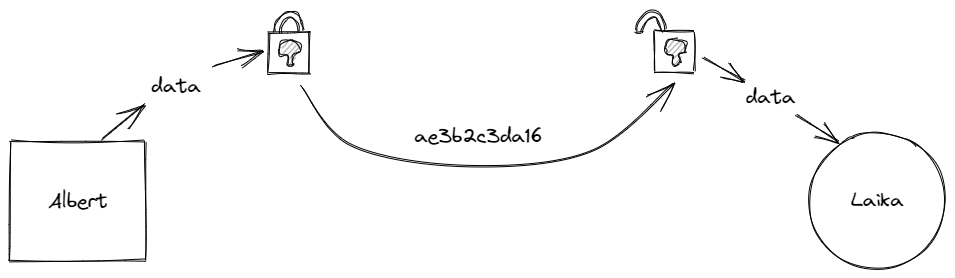
\includegraphics[width=0.7\textwidth]{Figures/transport-encryption.033b6a51.png}
        \caption{En esta figura, tenemos dos peers, que quieren enviar una información. IPFS \cite{web:ipfs} encripta directamente la información haciendo imposible ver los datos \textbf{cuando están viajando de nodo en nodo}.}
        \label{fg:trasnporte}
    \end{figure}
\end{center}
\subsection{Contenido}
La encriptación de contenido \ref{fg:contenido}, se utiliza cuando cuando se quiere asegurar que solo que alguien que tiene la contraseña, puede acceder al contenido.
\begin{center}
    \begin{figure}[h!]
        \centering
        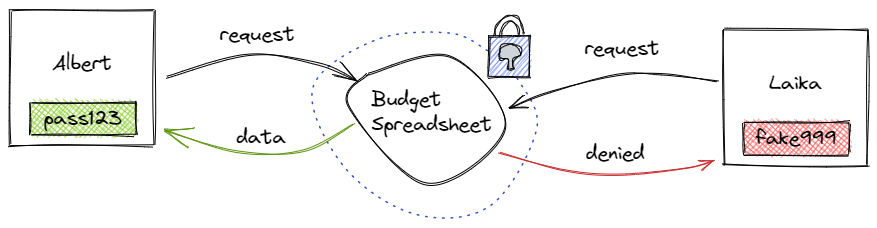
\includegraphics[width=0.7\textwidth]{Figures/content-encryption.adc5de58.png}
        \caption{En la figura, sin la contraseña correcta, Laika no puede acceder al fichero.}
        \label{fg:contenido}
    \end{figure}
\end{center}
IPFS \cite{web:ipfs} usa encriptación de transporte \ref{fg:trasnporte}, pero no encriptación de contenido \ref{fg:contenido}. Esto, según su wiki, se hace para que no exista un bias a la hora de elegir que tipo de encriptación es mejor para cada proyecto.
Para este proyecto, se han seleccionado una combinación de criptografía asimétrica con criptografía simétrica.
\subsection{XSalsa20 - Criptografía asimétrica}
La \textbf{criptografía asimétrica} (en inglés asymmetric key cryptography), \textbf{criptografía de clave pública} (en inglés public key cryptography) o \textbf{criptografía de dos claves} (en inglés two-key cryptography), es un sistema para poder compartir información utilizando claves publicas y privadas. Las claves publicas, como su nombre indica, son accesibles por todo el mundo. En cambio, la clave privada, tiene que permanecer protegida. \cite{web:asimetrica}
\begin{figure}[h!]
    \centering
    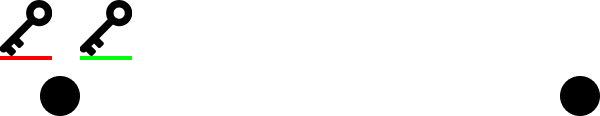
\includegraphics[width=0.7\textwidth]{Figures/Claves.png}
    \caption{Clave publica señalada en verde y la clave privada en rojo.}
    \label{fg:clave}
\end{figure}
Cuando el nodo de la derecha quiere enviar información a la cual solo va a tener acceso el nodo de la izquierda, tiene que usar su clave publica. \ref{fg:clave}
\begin{figure}[h!]
    \centering
    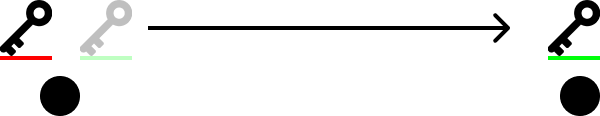
\includegraphics[width=0.7\textwidth]{Figures/Claves en movimiento(1).png}
    \caption{El host de la izquierda comparte su clave pública con el host de la derecha}
    \label{fg:movimiento}
\end{figure}
El nodo de la derecha, introducirá el mensaje en una caja y cerrara el candado utilizando esa llave. Ese candado, solo puede ser abierto por la clave privada perteneciente al par original. \ref{fg:movimiento}
\begin{figure}[h!]
    \centering
    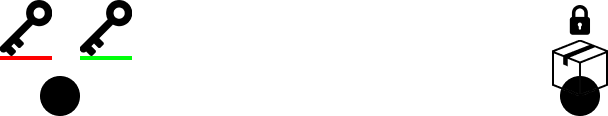
\includegraphics[width=0.7\textwidth]{Figures/Caja.png}
    \caption{El host de la derecha crea una \textit{caja}}
\end{figure}
Por ultimo lo único que queda, es enviar esa caja a su destinatario, lo cual se puede realizar por IPFS \cite{web:ipfs} de manera segura.
TweetNaCl \cite{web:tweetnacl}, o “sal”, es una librería que consigue reducir el tamaño de NaCl. Haciéndolo igual de rápido pero haciendo que su código fuente quepa en 100 tweets. De ahí su nombre.
\begin{quote}
    \textbf{Matthew D. Green, 2012}\\
    OpenSSL is the space shuttle of crypto libraries. It will get you to space, provided you have a team of people to push the ten thousand buttons required to do so. NaCl is more like an elevator—you just press a button and it takes you there. No frills or options.\\
    I like elevators. \cite{web:tweetnacl_elevator}
\end{quote}
\subsection{AES - Criptografía simétrica}
Aunque en teoría todas las comunicaciones se podrían hacer a través de criptografía asimétrica, para poder encriptar y desencriptar, como esas claves son las de la cartera del usuario, estamos limitados por el tamaño máximo que puedan soportar. Tenemos que comunicarnos con su cartera ya que nunca hay que dar la clave privada a nadie. Las claves privadas son propias y siempre deben serlo.
La criptografía simétrica se basa en una simple clave. Cualquier entrada se puede encriptar y des encriptar con la misma clave. Para eso, a la hora de crear la caja para el usuario, generamos una contraseña aleatoria utilizando la api crypto del navegador.
\begin{lstlisting}
    window.crypto.randomUUID()
\end{lstlisting}
\begin{quote}
    9fc2a1d0-5345-464c-a81e-a57a06b67669
\end{quote}
Después de esto se sigue el siguiente flujo.
\begin{itemize}
    \item Se encripta el fichero utilizando las apis nativas de los navegadores.
    \item Anunciamos la existencia de un nuevo fichero en nuestro nodo de IPFS \cite{web:ipfs}.
    \item En la caja introducimos el CID del fichero y la contraseña encriptada con la clave publica.
    \item Por ultimo anunciamos por pub sub que se ha subido un fichero y que el destinatario puede abrirlo.
\end{itemize}
Para esta parte del proyecto se ha elegido AES ya que es muy popular y esta soportado y tiene un buen historial de seguridad.
\newpage
\thispagestyle{empty}